\documentclass[11pt]{article}

\usepackage[estonian]{babel}
\usepackage[utf8]{inputenc}
\usepackage{amsmath}
\usepackage{tikz}
\usepackage{graphicx, wrapfig}
\usepackage[per-mode=symbol, decimalsymbol=comma, exponent-product = \cdot]{siunitx}
\usepackage{enumerate}
\usepackage{physics}
\usepackage[margin=2.5cm]{geometry}
\usepackage{lmodern, microtype}
\usepackage{hyperref}

\setlength\parindent{0pt}

\newcommand{\yl}[1]{\noindent{\bf Ülesanne #1} \quad}
\newcommand{\lah}{\noindent{\bf Lahendus} \quad}

\begin{document}
{\small Optika (LOFY.01.008) seminar \hfill kevad 2020}\\

{\Large Kodutöö XII}\\

Kui materjali lugedes või ülesandeid lahendades tekib küsimusi, siis pange need kirja ja esitage vastava osa õppejõule või seminaride läbiviijale Moorits Mihkel Murule (\texttt{moorits.mihkel.muru@ut.ee}). Kodutöö hinne kujuneb kahe parima lahenduse hindest. Tärniga ülesande lahenduse esitamine on kohustuslik.

\rule{\linewidth}{1pt} \\

\yl{1} Kõige lihtsamaks fotoaparaadiks (\textit{camera obscura} vt joonis \ref{cam}) on kinnine karp, mille tagaseina siseküljele on paigutatud fotopaber ja esiseina keskele on tehtud väike auk diameetrikga \(d\). Seesuguse nõelaaugu-kaamera fookuskaugseks \(f\) loetakse tagaseina kaugust esiseinast. Missugune on ava optimaalne läbimõõt \(d\), et kauge objekti kujutis oleks võimalikult terav. Arvutustes kasuta fookuskaugust \(f=\SI{10}{\centi\meter}\) ja lainepikkust \(\lambda=\SI{550}{\nano\meter}\).\\

\begin{figure}[!h]
	\centering
	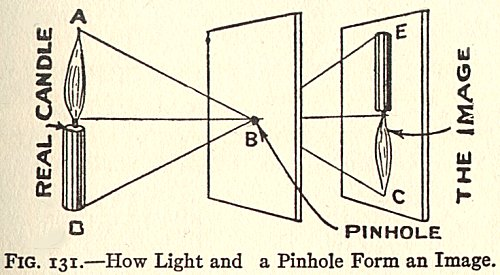
\includegraphics[width=0.5\textwidth]{camobs.jpg}
	\caption{\textit{Camera obscura} \small \url{http://www.uh.edu/engines/epi1772.htm}}
	\label{cam}
\end{figure}

\yl{2}  Kaks kõlarit, mis tekitavad ühesugust heli, asuvad üksteisest 15 cm kaugusel. Kõlaritest \num{1.25} meetri kaugusel on tilluke mikrofon, mis ristuvas teljes skaneeris joonisel \ref{kolar} toodud modulatsioonimustri. Heli kiirus õhus on 343 m/s. Leia kõlarite tekitatud helilainete ligikaudne sagedus. \\
\begin{figure}[!h]
	\centering
	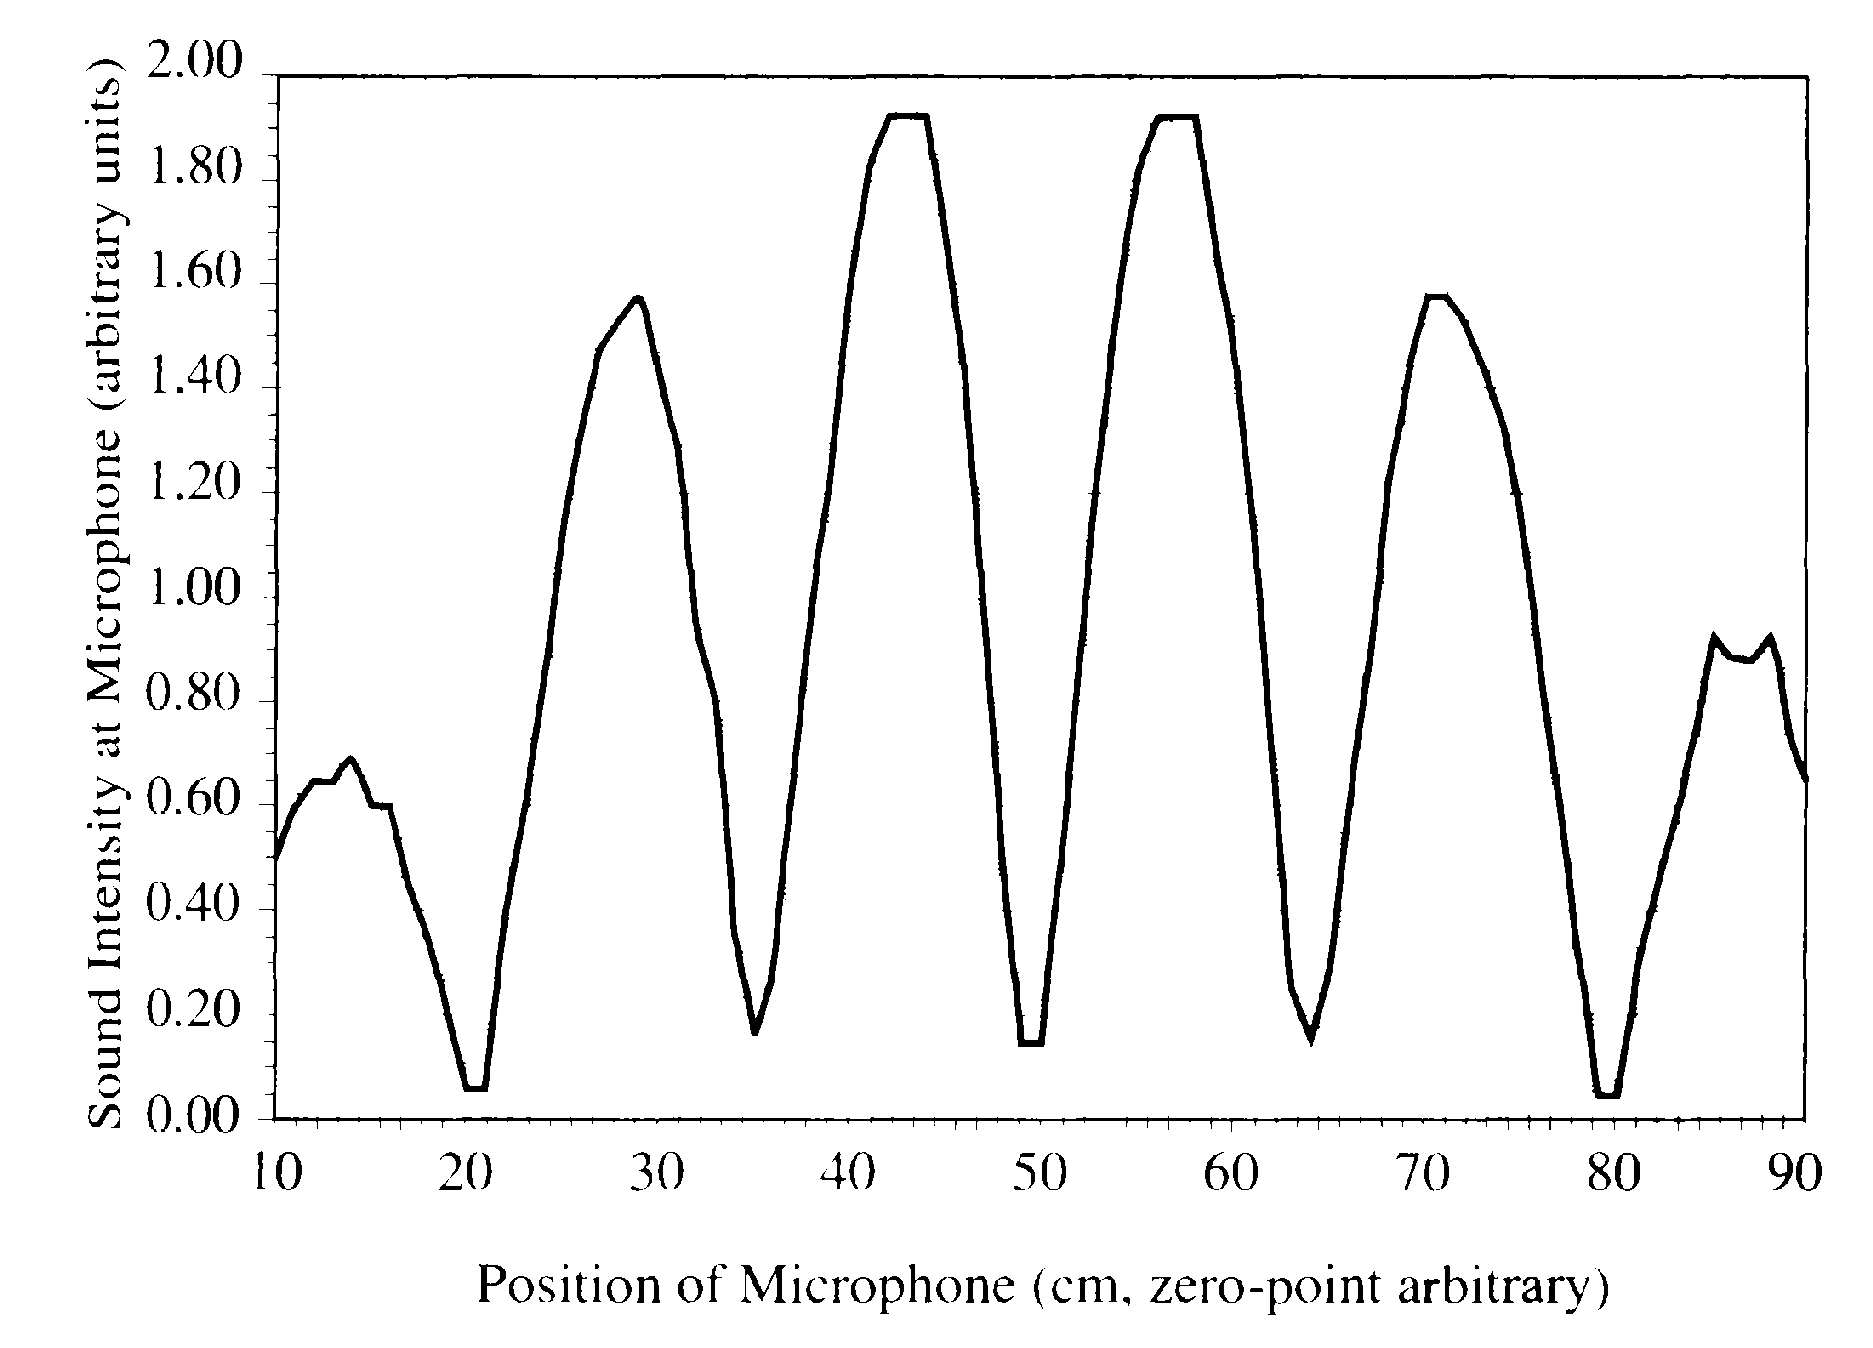
\includegraphics[width=0.8\textwidth]{kolarid.png} \\
	\caption{Mikrofoniga salvestatud helitugevus. \small \textit{Allikas: Hechti optika õpik}}
	\label{kolar}
\end{figure}

\yl{3} Avalda kiire nihe pärast tasaparalleelse klaasplaadi läbimist. Tee selgitav joonis. Lõpptulemus võib sõltuda plaadi paksusest, murdumisnäitajast ja nurgast plaadi pinnanormaali ja kiire vahel.\\

\yl{4*} Kirjelda joonis \ref{difraction} põhjal, mitme pilu difraktsiooniga on tegemist ja mis on pilu laiuse ning pilude omavahelise kauguse suhe. Tee joonis difraktsioonivõre intensiivsusest, millel on 8 pilu, laiusega \SI{200}{\micro\meter} ja nende omavaheline kaugus on \SI{600}{\micro\meter}.\\

\begin{figure}[!h]
    \centering
    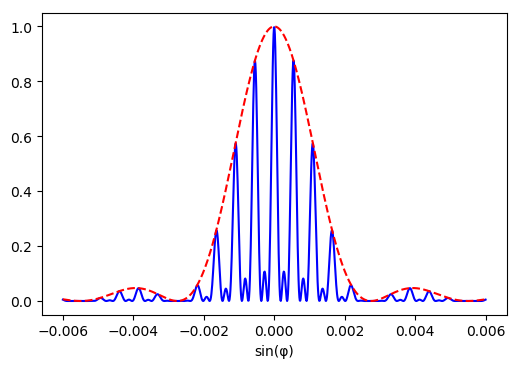
\includegraphics{difraction.png}
    \caption{Difraktsiooni intensiivsus (sinine) ja modulatsioon (katkendlik punane).}
    \label{difraction}
\end{figure}


\end{document}
